% コンパイルコマンド
% platex abs.tex
% dvipdfmx abs.dvi

\documentclass[a4j,9pt,twocolumn]{jsarticle}

%\usepackage{multicol} %2段組み用
\usepackage{amsmath}  %alignなど数式関係で必要になることが多い.
%\usepackage{graphicx} %図の取り込みに利用.
\usepackage[dvipdfmx]{graphicx} %図の取り込みに利用.
\usepackage{url}      %URLの表記に使う\urlコマンドに必要.
\usepackage{txfonts}  %英文をTimes Romanのようなフォントにする.
                      %通常のLaTeXのフォントにしたいときはこれをコメントアウトする.
\usepackage{algorithm,algorithmic} %algorithmとalgorithmic環境を利用するのに必要.
\usepackage{enumerate}%enumerate環境で項目を[Step 1.]のような形式に変更するのに利用.
\usepackage{ascmac} %itembox環境を利用するのに必要
\usepackage{longtable} 
\usepackage{multicol} % 複数列の箇条書き
\usepackage{enumitem}  % enumerateのインデントを調整

\pagestyle{plain} %ページ番号のスタイル
\urlstyle{same}   %\urlコマンドのフォント指定."tt", "rm", "sf", "same"(=使用中のフォント)

%%%%%%%%%%%%%%%%%%%%%%%%%%%%%% ↓テキスト幅,マージン,行間の調節
\textwidth     =  195mm %テキスト幅
\oddsidemargin = -7.5mm %左側のマージン
\textheight    =  280mm %テキストの高さ
\topmargin     =  -10mm %上のマージン
\renewcommand{\baselinestretch}{0.85} %行間を調節
%%%%%%%%%%%%%%%%%%%%%%%%%%%%%% ↑テキスト幅,マージン,行間の調節

%%%% ↓Change the style of itemize, enumerate, etc.
%%%% ↓(without space between items)
\makeatletter
\def\@listI{\leftmargin\leftmargini
    \topsep  \z@
    \parsep  \z@
    \itemsep \z@}
\let\@listi\@listI
\@listi 
\def\@listii{\leftmargin\leftmarginii
    \labelwidth\leftmarginii\advance\labelwidth-\labelsep
    \topsep  \z@
    \parsep  \z@
    \itemsep \z@}
\def\@listiii{\leftmargin\leftmarginiii
    \labelwidth\leftmarginiii\advance\labelwidth-\labelsep
    \topsep  \z@
    \parsep  \z@
    \itemsep \z@}
\makeatother
%%%% ↑Change the style of itemize, enumerate, etc.

%%%% ↓algotithmic の \REQUIRE と \ENSURE の表記を変更する
\renewcommand{\algorithmicrequire}{\textbf{Input:}}
\renewcommand{\algorithmicensure}{\textbf{Output:}}
%%%% ↑algotithmic の \REQUIRE と \ENSURE の表記を変更する

\newcommand\coleq{\mathrel{\mathop:}=}% \coleqの定義(:=をきれいに出力する)

\begin{document}
\pagestyle{empty} % ページ番号を表示しない.
\twocolumn[%
\begin{center}
 \vspace{-5mm}
 {\large \textbf{セキュアなV2Vアドホックネットワークルーティング
 プロトコルのための \\
 EdDSA署名方式の評価}}\\
 \vspace{2mm}
 {\large 工学部 電気電子・情報工学科 情報コース 三嶋研究室 永野正剛 } \\
\end{center}
\vspace{5mm}
]

\section{はじめに}
\textbf{VANET (Vehicle Ad hoc Network)}とは, 移動する車両間で通信を行うための
モバイルアドホックネットワークである. VANETの実用化には低遅延かつ高速な通信と
セキュリティの確保が求められる. しかし, セキュリティの確保には追加の処理が必要となるため, 
この処理をいかに効率化するかが問題となる. 階戸\cite{shinato}は, 既存のルーティングプロトコル
GPSRを改良し, 車両の位置情報とIPアドレスの詐称による不正を防ぐため, 
デジタル署名による認証を導入した. 以下, この改良版を「階戸のプロトコル」と呼ぶ. 
階戸は, 署名方式にDSAとECDSAを用いてシミュレーションを行い, ECDSAがネットワークの拡大に
対する柔軟性 (スケーラビリティ)で優れていることを示した. 本研究では, 階戸のプロトコルの
更なる効率化を目指し, 安全性はECDSAと同等以上で, 計算効率はECDSAより良いとされる署名方式
EdDSA (Edwards-curve Digital Signature Algorithm)を組み込むことにした.  
その性能を階戸のプロトコルと比較して評価するため, 離散型ネットワークシミュレータ ns-3用いて, 
ネットワークへの負荷や同一エリア内のノード数に対する拡張性を調査するシミュレーション実験を
行った. 
\section{関連技術, 関連研究}
\noindent \textbf{(1) GPSR}\\
\indent \textbf{GPSR (Greedy Perimeter Stateless Routing)}\cite{gpsr}は, ノードの位置情報と
IPアドレスを用いるルーティングプロトコルである. 各ノードは, 以下の処理を行い, 
ルーティングを構築する. 
\begin{itemize}
\item 自身の位置情報とIPアドレスを載せたHelloパケットを一定間隔で
ブロードキャストする.
\item 受信したHelloパケットの情報を用いて隣接ノードテーブルを更新する.
\end{itemize}

\noindent\textbf{(2) EdDSA}\\
\indent \textbf{EdDSA}は,  2011年にBernsteinら\cite{eddsa}
によって提案され, 近年標準化された比較的新しいデジタル署名方式である. 
EdDSAは, ECDSAに比べて演算が高速で, シンプルかつセキュアであるという特徴を
もつ. 特に, EdDSAのバリエーションの1つであるEd25519は, その効率性と安全性から
, ブロックチェーンや通信プロトコル, 認証システムなどでも採用されるなど
広く利用されるようになってきている. 以下にECDSAと比較したEdDSAの
特徴を, セキュリティと処理時間の観点から示す.
\smallskip
\begin{description}[labelwidth=3mm, labelsep=2mm]
    \item[(i)] \textbf{秘密鍵の安全性}\\
    ECDSAでは, 署名生成に使用する乱数が予測可能または重複した場合, 
    数学的な式変形によって秘密鍵を直接計算できるリスクがある. 一方. EdDSAでは, 
    署名生成に使用する乱数は, メッセージと秘密鍵を入力としたハッシュ値であるため, 
    乱数の漏洩したとしても, ハッシュ関数の原像計算困難性より, 
    秘密鍵を直接求めることができない. 


    % ECDSAでは、署名生成に使用される乱数(nonce)がランダムに生成されるため、  
    % もし乱数が予測可能であったり、異なるメッセージ間で同じ乱数が再利用された場合、  
    % 数学的な式変形によって秘密鍵を直接計算できるリスクがある。  
    % これにより、ECDSAのセキュリティは乱数の生成の安全性に大きく依存しており、  
    % 乱数の管理が適切に行われないと致命的な脆弱性となる。  

    % 一方、EdDSAでは、署名生成に使用する乱数 `r` は、メッセージと秘密鍵をハッシュ関数に  
    % 入力して計算することで決定論的に生成される。これにより、乱数の予測や重複の問題を防ぐことができる。  

    % しかし、EdDSAのセキュリティが優れている本質的な理由は、この決定論的な性質ではなく、  
    % 署名計算の設計にある。EdDSAの署名 `(R, S)` は、追加のハッシュ関数 `H(R, 公開鍵, メッセージ)` を含む形で  
    % 計算されるため、仮に `r` の値が漏洩したとしても、秘密鍵 `d` を直接求めることができる数式が存在しない。  
    % そのため、ECDSAのように乱数 `r` が攻撃者に知られたり重複したりしても、秘密鍵の漏洩につながることはない。  

    % つまり、EdDSAは**「決定論的な乱数生成」によって乱数管理の失敗を防ぐ**だけでなく、  
    % **「署名計算の設計」自体が乱数の漏洩を許容できる構造となっている**ため、ECDSAに比べて  
    % セキュリティ上のリスクが大幅に低減されている。  
\end{description}
\smallskip
\begin{description}[labelwidth=3mm, labelsep=2mm]
    \item[(ii)] \textbf{乱数生成の回避}\\
    一般的に, 暗号的に安全な乱数は, 生成の時間がランダムで処理コストが高い.
    EdDSAでは乱数を鍵生成でのみ使用しており, 署名生成, 署名検証では
    乱数を使用しない. そのため, 署名の生成と検証が一定時間で行われ, 乱数を使用するアルゴリズムに比べて
    高速に処理することができる.
\end{description}
\smallskip
\begin{description}[labelwidth=3mm, labelsep=2mm]
    \item[(iii)] \textbf{乗法逆元計算の回避}\\
    EdDSA (Ed25519)では, 拡張した射影座標系(拡張ツイストエドワーズ座標)で
    計算することがRFC8032 \cite{8032}で推奨されている.
    この座標系の特性により, 処理コストの高い乗法逆元の計算が不要となる.
    したがって, 処理が単純化され,  高速化しやすい. 
\end{description}
\smallskip
\noindent\textbf{(3) 階戸のプロトコル}\\
\indent GPSRでは, 同一アドホックネットワークの参加者が相互に正しい位置情報を
送信しない限り, ルーティングが正しく行われない. そのため, 
階戸のプロトコル\cite{shinato}では, ノード情報にデジタル署名を付与することで
なりすましや改ざんを排除している. 具体的には, 送信者がノード情報 
(IPアドレス, 位置情報)の正当性を担保する認証機関からの署名をHelloパケットに
付加して送信し, 受信者はそれらの署名の検証に成功した場合のみノードテーブルを
更新する(図\ref{fig:introduce}). 
署名者 (認証機構)と被署名データの対応を表\ref{tab:sign}に示す. 
\vspace{-3mm}
\begin{table}[h]
    \centering
    \caption{署名者と被署名データの対応\cite{shinato}}
    \label{tab:sign}
    \begin{tabular}{cc} \hline
        署名者 & 被署名データ \\ \hline \hline
        DHCPサーバ & IPアドレス \\
        位置情報認証機関 & 位置情報 \\ \hline
    \end{tabular}
\end{table}
\vspace{-5mm} % ← ここで表と図の間の余白を詰める
\begin{figure}[h]
    \centering
    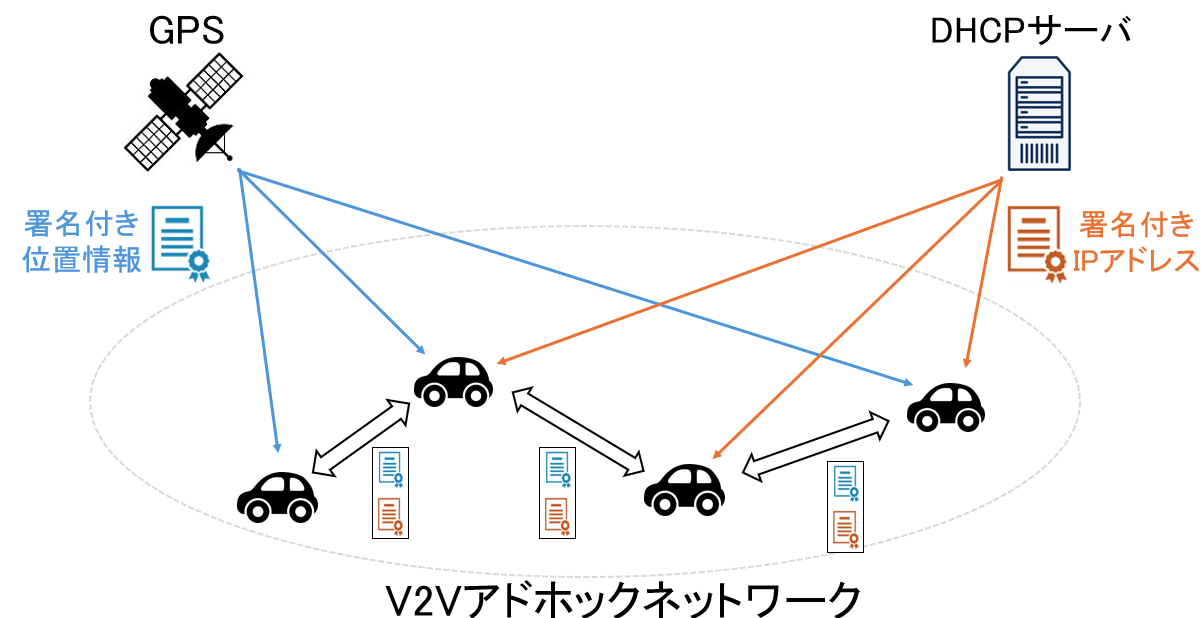
\includegraphics[width=0.45\textwidth]{figures/introduce.png}
    \caption{階戸のプロトコル\cite{shinato}}
    \label{fig:introduce}
\end{figure}
\vspace{-5mm}
\section{提案手法}
\indent 本研究では, 階戸のプロトコル\cite{shinato}をもとに, 署名方式を
EdDSAに差し替え, その通信効率を評価することを目的として, 次の2つのことを行った.\\ 
\noindent\textbf{(1) EdDSAの導入}\\
\indent EdDSAの最も一般的な実装であるEd25519を階戸のプロトコルにおける
署名方式と差し替え, 階戸と同様のシミュレーション環境でシミュレーション実験を行った. 
階戸は, ns-3のGPSRのモジュールにOpen SSLのDSAとECDSAの署名機能を追加する
コーディング行っていた. 本研究では, EdDSAを導入するために, Open SSLのEd25519の署名機能を
GPSRモジュールに追加するようコーディングを行った. \\
\noindent\textbf{(2) 評価基準の選定}\\
\indent 以下の8項目の評価基準により, ECDSAとEdDSAの2つの署名方式の違いによる
性能差を評価する.  なお, 遅延時間は中央値と最頻値, その他は平均値を用いる.
\vspace{-3mm}
\setlength{\columnsep}{10pt} % デフォルトは約35pt
\begin{multicols}{2}
    \begin{enumerate}
        \item スループット 
        \item 遅延時間 (Delay)
        \item パケット配送率 (PDR)
        \item オーバーヘッドサイズ\\
        \item シミュレーション実行時間
        \item 署名作成時間
        \item 署名検証時間
        \item メモリ使用量
    \end{enumerate}
\end{multicols}
\vspace{-3mm}
\section{シミュレーション実験}
\indent 本研究では, ns-3を用いて3つのシミュレーション実験を行った.  
いずれの実験でも, 以下の4パターンについて調べた. 
\begin{itemize}
    \item 認証機構を用いない場合
    \item DSAを用いて認証機構を追加した場合
    \item ECDSAを用いて認証機構を追加した場合
    \item EdDSAを用いて認証機構を追加した場合
\end{itemize}
\indent 主要なシミュレーションパラメータを表\ref{tab:parameter}に示す. 

\begin{table}[h]
  \centering
  \caption{シミュレーションパラメータ}
  \label{tab:parameter}
  \begin{tabular}{ll} \hline
    シミュレーションツール & ns-3.26 \\
    通信規格 & IEEE 802.11p \\
    通信プロトコル & UDP \\
    パケットサイズ & 1024 [byte] \\
    パケット送信間隔 & 1.0 [s] \\
    送信電力 & 17.026 [dBm] \\
    電力検出閾値 & -96.0 [dBm] \\
    電波伝搬減衰モデル & 対数距離電波伝搬減衰モデル \\
    遅延モデル & 定常速度伝搬モデル \\
    電波伝搬範囲 & 約300 [m] \\
    ノード数 & 74 (実験1, 2)\\
    シミュレーション時間 & 300 [s] \\
    ルーティングプロトコル & GPSR \\
    デジタル署名 & DSA, ECDSA, EdDSA \\ \hline
  \end{tabular}
\end{table}
\subsection{実験1}
実験1では, 認証機構が正しく機能していることを確認するための実験を行った. 
全ノードの8\%を不正ノードとして設定し, 250回のシミュレーションを行った. 
導入する不正ノードは次の2種類である. 
\begin{enumerate}
    \item 位置情報を詐称するノード (4\%)\\
    通信データの窃取を目的に, 偽装した位置情報をHelloパケットで送信する不正ノード. 
    \item IPアドレスを詐称するノード (4\%)\\
    不正アクセスを目的に, 偽装したIPアドレスをHelloパケットで送信する不正ノード. 
\end{enumerate}
\medskip
 実験1の結果を表\ref{tab:exp1}に示す.
\begin{table}[h]
    \centering
    \caption{実験1のシミュレーション結果}
    \label{tab:exp1} 
    \begin{tabular}{l|crrr} \hline
        評価基準 & 認証無し & DSA & ECDSA & EdDSA \\ \hline \hline
        PDR[\%] & $48.2$ & $88.15$ & $86.62$ & $84.48$ \\
        Throughput[kbps] & $4.18$ & $7.64$ & $7.51$ & $7.33$ \\ \hline
    \end{tabular}
\end{table}

表\ref{tab:exp1}から, 認証機構を追加したプロトコルは, 署名方式に依らず
パケット配送率 (PDR)とスループット (Troughput)が同程度向上していることがわかる. 
署名方式の違いによる差異はないため, 3つの署名方式は同等のセキュリティ性能を
もつと考えられる. 

\subsection{実験2}
\indent 実験2では, 認証機構の追加が通信にどれだけの負荷を与えるかを調査するため, 
不正ノードの存在しない環境で, 250回のシミュレーションを行った. \\
\indent 実験2の結果を表\ref{tab:exp2}に示す. 
\vspace{-3mm}
\begin{table}[h]
    \centering
    \caption{実験2のシミュレーション結果}
    \label{tab:exp2} 
    \begin{tabular}{l|rrrr} \hline
        評価基準 & 認証無し & DSA & ECDSA & EdDSA \\ \hline \hline
        \footnotesize{median of Delay[ms]} & $6.88$ & $6.13$ & $6.20$ & $84.48$ \\
        \small{mode of Delay[ms]} & $[6.0, 7.0)$ & $[2.0, 3.0)$ & $[2.0, 3.0)$ & $[6.0, 7.0)$ \\
        PDR[\%] & $83.21$ & $87.80$ & $86.89$ & $87.39$ \\
        Overhead[KB] & $2694.3$ & $5982.8$ & $5384.2$ & $5364.5$ \\ \hline
    \end{tabular}
\end{table}

表\ref{tab:exp2}から, 遅延時間は経路選択のタイミングによって左右されるため, 
若干の差異が出てしまうが, 認証機構の有無が遅延時間に影響を与えないことがわかる. 
また, 認証機構の有無はパケット配送率に影響を与えないことがわかる. 
オーバーヘッドサイズは, 認証機構を追加することで,大幅に増加している. これは, Helloパケットの
データに署名が付与されていることが原因である. また, 署名方式の違いによる差は, 各署名方式で
用いられる鍵長が原因であると考えられる. なお, 本研究で使用したパラメータによる
それぞれの鍵長は, 同程度の安全性が保証されるよう, DSAで2048ビット, ECDSAとEdDSAで256ビットとした. 

\subsection{実験3}
\indent 実験3では, 同一エリア内のノード数に対する拡張性を調査するため, 
不正ノードの存在しない環境でノード数を37, 74, 112, 148, 185に設定し, 
それぞれ250回ずつシミュレーションを行った. \\
\indent 実験3の結果を表\ref{tab:exp3_simtime}, 表\ref{tab:exp3_sig}, 
表\ref{tab:exp3_memory}に示す. 
\begin{table}[h]
    \centering
    \caption{ノード数によるシミュレーション実行時間}
    \label{tab:exp3_simtime}
    \begin{tabular}{c|rrrr} \hline
        ノード数 & \multicolumn{4}{c}{シミュレーション実行時間 [s]} \\ \cline{2-5}
                       & 認証無し & DSA & ECDSA & EdDSA \\ \hline \hline
        37  &  14.18  &   69.99  &   55.01  &   24.41  \\
        74  &  50.60  &  267.43  &  194.41  &   89.27  \\
        112 & 110.41  &  625.50  &  436.93  &  200.90  \\
        148 & 196.97  & 1172.57  &  910.37  &  431.35  \\
        185 & 345.06  & 1908.70  & 1324.55  &  635.16  \\ \hline
    \end{tabular}
\end{table}
\vspace{-5mm}
\begin{table}[h]
    \centering
    \caption{実験3のシミュレーション結果}
    \label{tab:exp3_sig} 
    \begin{tabular}{c|rr} \hline
        評価基準 & ECDSA & EdDSA \\ \hline \hline
        署名生成時間[ms] & $0.371$ & $0.031$ \\
        署名検証時間[ms] & $0.336$ & $0.097$ \\ \hline
    \end{tabular}
\end{table}
\vspace{-5mm}
\begin{table}[h]
    \centering
    \caption{ノード数によるメモリ使用量}
    \label{tab:exp3_memory}
    \begin{tabular}{c|cccc} \hline
        ノード数 & \multicolumn{4}{c}{メモリ使用量 [KB]} \\ \cline{2-5}
                       & 認証無し & DSA & ECDSA & Ed25519 \\ \hline \hline
        37  &  70,939.4  &  72,023.3  &   93,749.3  &   80,647.1  \\
        74  &  74,089.7  &  74,989.3  &  151,853  &  106,442  \\
        112 &  77,070.1  &  78,134.7  &  254,247  &  151,401  \\
        148 &  80,749.9  &  81,752.5  &  409,965  &  219,102  \\
        185 &  84,548.1  &  85,541.4  &  560,753  &  285,191  \\ \hline
    \end{tabular}
\end{table}
\vspace{-3mm}
  
\indent ECDSAとEdDSAに注目して結果を評価すると, EdDSAの方が実行時間, 署名の生成と
検証の時間が短く, メモリ使用量も小さかった. これらの結果は, EdDSAがECDSAよ
りもスケーラビリティに優れていることを示唆している. 

\section{まとめと今後の課題}
\indent 実験結果の評価から, EdDSAはECDSAよりも計算効率が高いことが確かめられた. 
これは, EdDSAの設計上の特徴である高速な処理能力が実験環境においても十分に発揮されたことを
示している. したがって, 階戸のプロトコルにおいて, EdDSAはECDSAよりも効率的な
認証方式として利用できるといえる. \\
\indent 今後は, 送受信ノードの数やノードの動き,通信のリンク状況などの要件を変更して
シミュレーションを行い, 多様な実験環境での影響を調べ, EdDSAのVANETへの
適用可能性の調査を進めるとともに, より効率的な認証方法の探求も進めていきたい. 




\noindent\hrulefill % 参考文献の上に線を引く
%%%%%%%%%%%%%%%%%%%%%%%%%%%%%%%%%%%%%%%%%%%%%%%%%%%%%%%%%%%% References
\begin{thebibliography}{99}
    \bibitem{shinato} 階戸 弾,
        \textit{デジタル署名を用いたセキュアなV2Vアドホックルーティングプロトコル},
            岐阜大学大学院自然科学技術研究科修士論文, 2024.
    \bibitem{8032} Simon Josefsson and Ilari Liusvaara, 
        RFC 8032: Edwards-Curve Digital Signature Algorithm (EdDSA),
        Internet Engineering Task Force (IETF), 
        https://tex2e.github.io/rfc-translater/html/rfc8032.html, 
        2017.
    \bibitem{gpsr} Brad Karp and H. T. Kung, 
        \textit{GPSR: Greedy Perimeter Stateless Routing for Wireless Networks},
        Proceedings of the 6th annual international conference on Mobile computing and networking,
        pp. 243-254, 
        2000.
    \bibitem{eddsa} Daniel J Bernstein, Niels Duif, Tanja Lange, Peter Schwabe, and Bo-Yin Yang,
        \textit{High-speed high-security signatures}, Journal of Cryptographic Engineering,
        2-17, 2011.
\end{thebibliography}

%%%%%%%%%%%%%%%%%%%%%%%%%%%%%%%%%%%%%%%%%%%%%%%%%%%%%%%%%%%%
\end{document}










% \section{まとめ}
% 通常の論文等ではこのように得られた成果をまとめた結論を書いて終わるのですが,
% 研究の進捗状況を報告する普段の研究会の発表では,結論を書くことは難しいかもしれません.
% また,既に一定の成果が得られている場合でも,卒論・修論の締切が差し迫った時期を除き,
% 卒論・修論に向けてさらに研究を進める予定であると思います.
% そのような場合には,この節のタイトルを例えば「まとめと今後の研究計画」などとして,
% まず現在までに得られている成果をまとめたのち,
% 今後の研究計画を簡潔に書いてください.
